\subsubsection{Smarter Monte Carlo Sampling}
Multivariable integrals arise in Bayesian inference, quantitative finance, and uncertainty quantification.  When the number of variables, $d$ is more than a few, tensor product rules are impractical because the rate of convergence, $\Order(n^{-r/d})$, where $n$ is the number of sampling points, degrades catastrophically with $d$, even if $r$, the smoothness of the integrand and the associate method is substantial.  The most computationally efficient methods are Monte Carlo methods, where the integral of interest is interpreted as the expectation (or population mean) of a function of a (uniform) random variable, which is then approximated by a sample mean.
$
    \int_{\Omega} g(\bt) \, \dif \bt = \int_{[0,1]^d} f(\bx) \, \dif \bx = \Ex[f(\bX)] \approx \frac 1n \sum_{i=1}^n f(\bx_i).
$

The root mean square error using $\bx_1, \bx_2, \ldots \IIDSim \calu[0,1]^d$ is $\std(f(\bX)) n^{-1/2}$, which translates into a computational cost of $\Order(d\var(f(\bx))\varepsilon^{-2})$ to obtain an approximation with absolute error no greater than $\varepsilon$. The term $d$ accounts for the cost of evaluating $f$, which is assumed to be proportional to the number of variables, $d$.

There are several ways to decrease the cost of computing an acceptable approximation to the integral.  Quasi-Monte Carlo (QMC) methods \cite{DicEtal14a} replace IID sample points by low discrepancy (LD) sample points, such as Sobol' or lattice points, reduces the cost to $\Order(d\norm{f}\varepsilon^{-1+\delta})$ for arbitrarily small, positive $\delta$, where now the size of integrand is measured by a norm that requires a bit more smoothness than IID Monte Carlo. 

Multi-level methods write the integral for large or even infinite $d$ as a telescoping sum involving integrals of increasing dimension. 
For many problems of interest, such as those where $f$ represents the payoff of an exotic option, one can use a large number of samples for the terms with small dimension and a small number of samples for the terms with large dimension so that the total computational cost now loses its $d$ dependence and becomes $\Order(\norm{f}\varepsilon^{-1+\delta})$.
 
\begin{wrapfigure}{r}{0.56\textwidth}
	\centering
	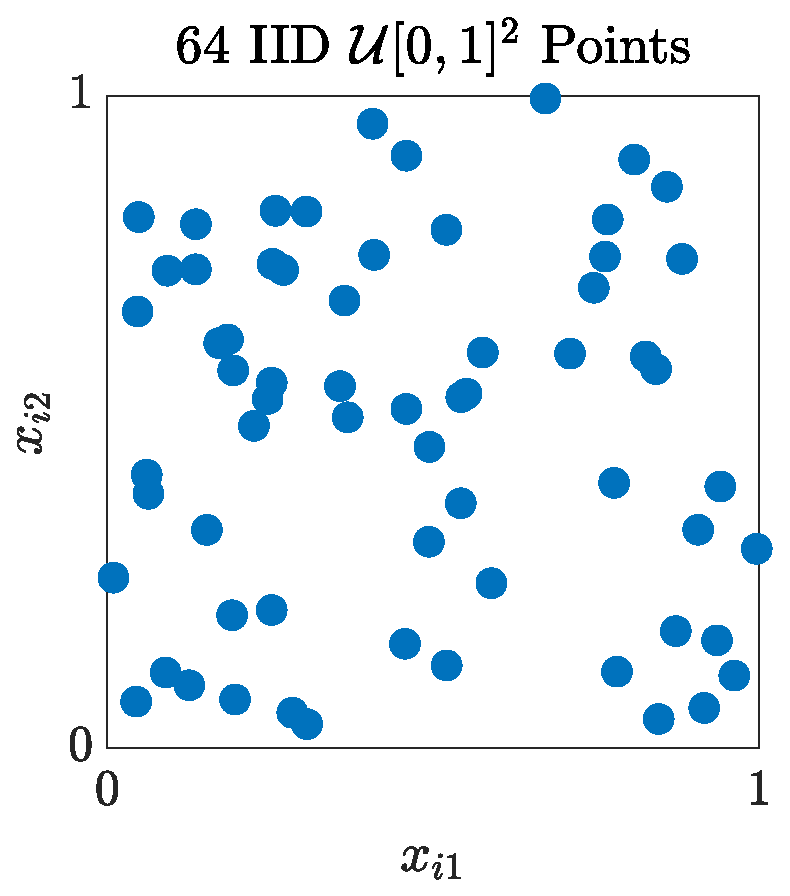
\includegraphics[height = 4.5cm]{IIDPoints.eps} \quad
	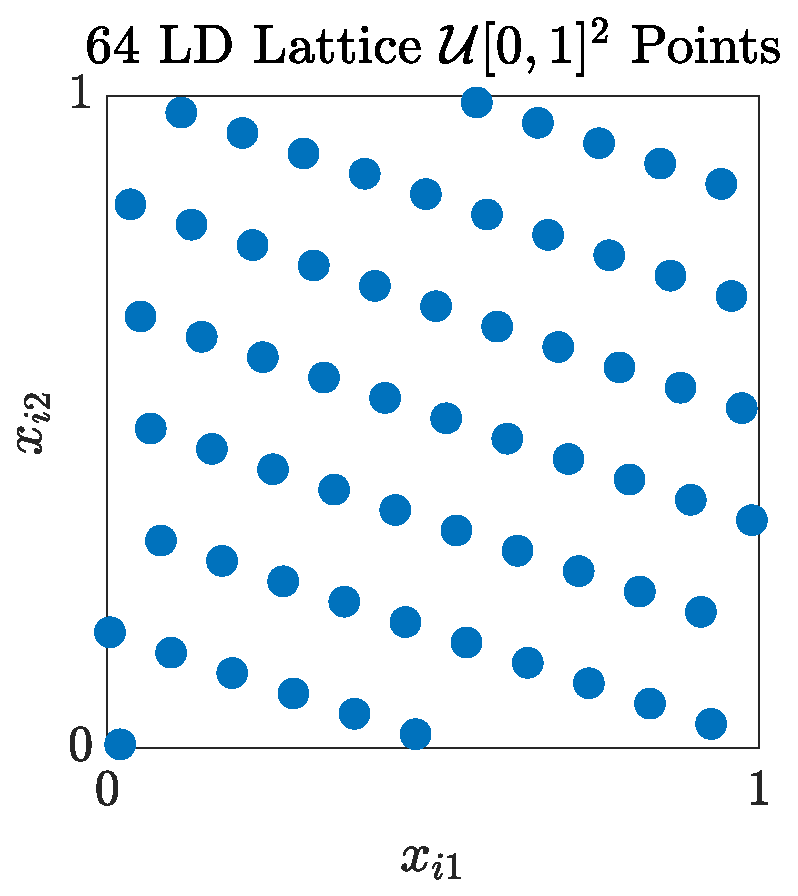
\includegraphics[height = 4.5cm]{ShiftedLatticePoints.eps}
	\caption{IID points and LD lattice points.  The LD points have fewer gaps and clusters of points than the IID points. \label{fig:iid_vs_ld}}
\end{wrapfigure}


Finally, the variable transformation from the original integral of $g$ to the final integral $f$ is non-unique.  Clever transformations, which may be regarded as importance sampling, make $\norm{f}$ smaller.  The integrands, $g$, in Bayesian inference problems are typically quite peaky, and importance sampling may drastically reduce the computational cost.

SURE students will explore one or more of these methods for more efficient Monte Carlo sampling in the context of QMCPy \cite{QMCPy2020a,QMCBlog}, an open-source quasi-Monte Carlo library developed by Hickernell, Choi, Ding, PhD student Sorokin and collaborators. The goal of the SURE projects will be to expand the menu of use cases for quasi-Monte Carlo, e.g., for efficient evaluation of acquisition functions in Bayesian Optimization and extending the work of Zhang \cite{Zha21a} in using QMC methods for Bayesian inference. 